% !TEX program = xelatex
\documentclass[10pt, a4paper]{ctexart}

\usepackage[left=1.0cm, right=1.0cm, top=1.0cm, bottom=1.0cm]{geometry}
\usepackage{titlesec}
\usepackage{graphicx}
\usepackage{enumitem}
\usepackage{hyperref}
\usepackage{xcolor}

% 设置超链接颜色
\definecolor{linkcolor}{HTML}{000000}
\hypersetup{
    colorlinks=true,
    linkcolor=linkcolor,
    urlcolor=linkcolor,
    citecolor=linkcolor
}

% 禁用段落缩进
\setlength{\parindent}{0pt}

% 自定义章节标题格式 (带有下划线)
\titleformat{\section}{\large\sffamily\bfseries}{}{0em}{}[\titlerule]
\titlespacing*{\section}{0pt}{0.6ex plus 0.5ex minus .1ex}{0.4ex plus .1ex}

% 自定义列表格式
\setlist[itemize]{leftmargin=1.5em, nosep, itemsep=0.1ex, topsep=0ex, parsep=0ex, partopsep=0ex}

\begin{document}
\pagestyle{empty}

% 头部信息 (左右两栏)
\begin{minipage}[c]{0.82\textwidth}
    {\huge \textbf{王嘉璇 (Wang Jiaxuan)}} \\[0.4em]
    华中科技大学 \quad $\cdot$ \quad 电子信息与通信学院 \quad $\cdot$ \quad 2027届本科 \\[0.2em]
    $|$ \textbf{电话} 18879965616 $|$ \textbf{邮箱} wangjx\_hust@hust.edu.cn $|$
\end{minipage}%
\begin{minipage}[c]{0.18\textwidth}
    \raggedleft
    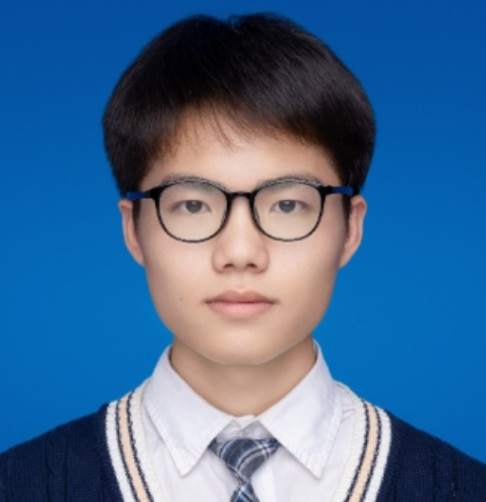
\includegraphics[width=3.2cm]{xun.jpg} 
\end{minipage}

\vspace{0.4em}

{\large \textbf{求学意向：直博}}

\vspace{0.4em}

\section{教育背景}
\textbf{华中科技大学}，电子信息与通信学院，电子信息工程专业，本科 \hfill 2023.9 - 2027.6\\[0.1em]
基于项目信息类专业教育实验班（“种子班”） \hfill 成绩：加权均分 \textbf{84.5/100} $|$ 排名 \textbf{Top 30\%} \\[0.1em]
高分核心课程：计算机与程序设计基础（C）（96分）、数字电子技术（92分）、随机过程（92分）、模拟电子技术（85分）、工程制图（一）（94分） \\[0.1em]
语言能力：CET-6 \textbf{519} 分，CET-4 \textbf{585} 分 \\[0.1em]
现任 \textbf{Dian团队 队长}；现任 \textbf{Dian团队 机器人组 组长}

\section{论文发表与学术会议}
\begin{itemize}
    \item Yefan Lin, \textbf{Jiaxuan Wang}, Baoyu Liu, Zheng Lv, and Xiaojun Hei, ``Pallet-ACT: A Unified Data-Training-Inference Framework for Industrial Robotic Palletizing.'' \textit{7th Information Communication Technologies Conference (\textbf{ICTC})}, Nanjing, China, May 2026. (\textbf{已通过初审})
    \item Yuhan Huang, Zijian Ning, Ziyuan Wang, \textbf{Jiaxuan Wang}, Xiaojun Hei, ``Reinforcement Learning with Stage-Wise Model Fusion for Sequential Object Manipulation Tasks.'' \textit{IEEE International Conference on Robotics and Biomimetics (\textbf{ROBIO})}, Chengdu, China, December 2025.
\end{itemize}

\section{技能与工具}
\begin{itemize}
    \item \textbf{编程语言}：熟练掌握 Python 与 C 语言。
    \item \textbf{机器人控制与真机实操}：具备丰富的 6轴机械臂真机实操、调试与部署经验；熟悉 ROS 2 机器人操作系统及 MoveIt 2 运动规划框架；掌握强化学习（RL）与模仿学习（IL）等 AI 算法在机器人控制与实际任务中的落地应用。
    \item \textbf{仿真与三维建模}：熟练应用 MuJoCo 物理引擎进行机器人的物理仿真与测试；精通 SolidWorks 进行三维建模与产品结构设计，并具备丰富的 3D 打印实际操作经验。
    \item \textbf{开发环境与高效工具}：熟悉 Linux 操作系统环境；熟练使用 VSCode 等主流 IDE，熟悉 VMware 与 Anaconda 等开发与环境管理工具；善于运用各类现代化 AI 工具辅助编程、文档编写与科研，具备极高的开发效率。
\end{itemize}

\section{竞赛与科研项目经历}
\textbf{ICRA 2025 Sim2Real 挑战赛} | \textbf{国际级二等奖}（全球第四名）
\begin{itemize}
    \item 作为团队DianRobot核心成员，在复杂连续物体操作赛道中展现了出色的仿真到现实迁移能力与算法控制水平
\end{itemize}

\vspace{0.2em}
\textbf{基于模仿学习的化学实验机械臂智能应用设计} | \textbf{省级大创项目 (在研)} \hfill 2025年度
\begin{itemize}
    \item 作为项目核心骨干及负责人，全程深度参与项目推进，负责机械臂对化学实验器材的精准抓取。(指导教师：黑晓军)
\end{itemize}

\vspace{0.2em}
\textbf{强化学习赋能机器人咖啡服务应用设计} | \textbf{中南地区赛本科组二等奖} \hfill 2024年
\begin{itemize}
    \item 通过视觉补偿解决了机器人抓取咖啡杯时的关节零漂问题，采取包围盒的方案实现了手指定位与抓取成功判定。
\end{itemize}

\vspace{0.2em}
\textbf{基于强化学习机器人做咖啡} | \textbf{校企合作横向项目 (已结题)} \hfill 2023.07 - 2024.04
\begin{itemize}
    \item 参与达闼机器人有限公司横向项目，参与机器人咖啡服务的设计与系统研发，完成做咖啡对外展示流程的搭建。
\end{itemize}

\vspace{0.2em}
\textbf{Dian团队接待机器人应用设计} | \textbf{校级大创项目 (结题优秀)} \hfill 2023年度
\begin{itemize}
    \item 参与接待机器人的全流程应用设计工作，舞蹈动作设计与编排。(指导教师：黑晓军/张成伟)
\end{itemize}

\vspace{0.2em}
\textbf{嵌入式系统课程设计：智能加热杯垫} | \textbf{核心开发者} \hfill 2025.9 - 2026.3
\begin{itemize}
    \item 参与智能加热杯垫总体软硬件开发，并主导外壳与结构设计；熟练运用 \textbf{SolidWorks} 等工具完成外壳开发。
\end{itemize}

\section{其他教学与工程项目参与经历}
\begin{itemize}
    \item \textbf{核心课程建设项目}：参与卓越工程师培养《服务机器人应用设计》课程建设（2026.1-2027.12，\textbf{在研}）。
    \item \textbf{教材建设项目}：参与卓越工程师培养《服务机器人应用系统设计与实验》教材编写与建设（2026.1-2027.12，\textbf{在研}）。
    \item \textbf{教学研究项目}：参与“基于深度产教融合的本研贯通专业学位研究生机器人体系”教研项目（2025.1-2026.12，\textbf{在研}）。
\end{itemize}

\end{document}
